\documentclass[10pt,twocolumn]{article}
\usepackage[utf8]{inputenc}
\usepackage[T1]{fontenc}
\usepackage{amsmath,amssymb}
\usepackage{graphicx}
\usepackage{booktabs}
\usepackage{multirow}
\usepackage{caption}
\usepackage[margin=2cm]{geometry}
\usepackage[hidelinks]{hyperref}
\usepackage{authblk}

\renewcommand{\thesection}{\Roman{section}}
\renewcommand{\thesubsection}{\thesection.\Alph{subsection}}
\setlength{\columnsep}{0.8cm}
\captionsetup{font=small}

\title{\vspace{-1.0cm}\textbf{Improving GANs using Optimal Transport}\\
\large A corrected, reproducible and measurable re-implementation}
\author[]{Dan Allouche}
\author[]{Nicolas Dahan}
\affil[]{\small ENSAE Paris, Palaiseau, France \\ \texttt{dan.allouche@ensae.fr} \quad \texttt{nicolas.dahan@ensae.fr}}
\affil[]{\footnotesize Originally ENSAE coursework (2021); corrected, modernized and extended (2026)}
\date{}

\begin{document}
\maketitle

\begin{abstract}
\noindent We reproduce the OT-GAN of Salimans et al.~\cite{salimans2018} on MNIST.
Beyond the original implementation, we identify and fix five correctness issues in the
training procedure---most importantly, the critic was optimized in the \emph{wrong
direction}---and we make the code device-portable (CPU/MPS/CUDA), numerically stable
(log-domain Sinkhorn) and quantitatively measurable. Under an upgraded evaluation
protocol (FID, KID and a domain-aware FID-LeNet, all at 10{,}000 samples), the
critic-sign fix alone \emph{divides the FID by $\approx 2.5$} (177.9 $\rightarrow$ 70.8),
turning formless blobs into clearly recognizable digits. We then modernize the
objective: replacing the mini-batch energy distance by a \emph{debiased} Sinkhorn
divergence~\cite{genevay2018,feydy2019} removes the documented critic collapse and
improves the FID from 81.2 to 24.4 at equal budget, and an optimal-transport
conditional flow-matching model~\cite{tong2024} built on the \emph{same} Sinkhorn
solver reaches FID 11.4. Finally, we show that the same OT engine extends, unchanged,
from images to market data: an entropic scenario-reduction tool and a 1D OT-GAN for
heavy-tailed returns generation (Sec.~\ref{sec:finance}).
\end{abstract}

\section{Generative Modeling and Optimal Transport}
Richard Feynman said: \emph{``What I cannot create, I do not understand''}. Generative
modeling aims to learn a model of a complex data distribution so as to generate data
similar to it. Generative Adversarial Networks (GANs) train a generator $G$ that captures
the data distribution and a discriminator $D$ that distinguishes generated from real data;
$D$ defines a distance that $G$ minimizes to make its samples resemble the data.

To avoid the tractability problems of the primal optimal-transport formulation, Salimans
et al.\ use mini-batches and a learned cost, defining the \emph{mini-batch energy
distance}:
\[
\resizebox{\columnwidth}{!}{$\displaystyle
D^2(p,g) = 2\,\mathbb{E}[\mathcal{W}_{c_\eta}(\mathbf{X},\mathbf{Y})]
- \mathbb{E}[\mathcal{W}_{c_\eta}(\mathbf{X},\mathbf{X}')]
- \mathbb{E}[\mathcal{W}_{c_\eta}(\mathbf{Y},\mathbf{Y}')]
$}
\]
where $p$ is the data distribution, $g$ the generator distribution,
$\mathbf{X},\mathbf{X}'$ are independent mini-batches from $p$, and
$\mathbf{Y},\mathbf{Y}'$ independent mini-batches from $g$. The entropic optimal-transport
cost is $\mathcal{W}_{c_\eta}(\mathbf{X},\mathbf{Y}) = \inf_{M\in\mathcal{M}} \mathrm{Tr}[M C^\top]$,
with $\mathcal{M}$ the set of non-negative matrices whose rows and columns sum to one,
$C_{i,j}=c_\eta(\mathbf{x}_i,\mathbf{y}_j)$, and the learned cosine cost
\begin{equation}
c_\eta(\mathbf{x},\mathbf{y}) = 1 - \frac{v_\eta(\mathbf{x})\cdot v_\eta(\mathbf{y})}
{\lVert v_\eta(\mathbf{x})\rVert_2\,\lVert v_\eta(\mathbf{y})\rVert_2},
\nonumber
\end{equation}
where $v_\eta$ (the \emph{critic}) is a deep neural network. The generator
\textbf{minimizes} $D^2$ while the critic $v_\eta$ \textbf{maximizes} it.

\section{Related Work}
\paragraph{Sinkhorn divergences.} Entropic regularization makes mini-batch optimal
transport tractable on GPU~\cite{cuturi2013}. Genevay, Peyr\'e and
Cuturi~\cite{genevay2018} train generative models with the resulting \emph{Sinkhorn
divergence} $S_\varepsilon(p,g) = \mathcal{W}_\varepsilon(p,g) - \tfrac12
\mathcal{W}_\varepsilon(p,p) - \tfrac12 \mathcal{W}_\varepsilon(g,g)$, whose theoretical
properties (positivity, metrization of weak convergence) are established by Feydy et
al.~\cite{feydy2019} for the \emph{debiased} estimator with \emph{same-batch} self-terms
$\mathcal{W}(\mathbf{X},\mathbf{X})$. The mini-batch energy distance of Salimans et
al.~\cite{salimans2018} is exactly \emph{twice} a Sinkhorn divergence whose self-terms
are estimated with \emph{independent} mini-batches $\mathcal{W}(\mathbf{X},\mathbf{X}')$;
the distinction between independent- and same-batch self-terms is precisely what our loss
study in Sec.~\ref{sec:modern} isolates.
\paragraph{Mini-batch-OT flow matching.} Flow matching~\cite{lipman2023} trains a
velocity field by plain regression along straight noise-to-data paths; Tong et
al.~\cite{tong2024} pair noise and data through a mini-batch OT plan instead of
independently, which straightens the marginal flow and reduces integration error at
sampling time. The same Sinkhorn solver that prices mini-batches inside the 2018 GAN can
therefore power its 2024 successor. GANs themselves remain competitive when
modernized~\cite{huang2024}.
\paragraph{Evaluation methodology.} We follow current practice on metric pitfalls: KID as
an unbiased complement to FID~\cite{binkowski2018}, aliased-resizing artifacts in FID
pipelines~\cite{parmar2022}, the strong bias of FID at small sample
counts~\cite{chong2020}---the reason we re-evaluate at 10{,}000 samples rather than
2{,}048---and the comparability caveats of the large-scale GAN study of Lucic et
al.~\cite{lucic2018}.

\section{Implementation}
We implement the OT-GAN in PyTorch and train it on MNIST ($1\times 32\times 32$). The
\emph{generator} maps a latent vector to an image: a linear layer followed by a Gated
Linear Unit (GLU) reshaped to $512\times 8\times 8$, then two (nearest-neighbour upsample,
$5\times 5$ convolution, GLU) blocks, and a final convolution with a $\tanh$ output. The
\emph{critic} maps an image to a $32768$-dimensional embedding through three ($5\times 5$
convolution, Concatenated-ReLU) blocks, a flatten, and an $\ell_2$ normalization---the
normalization is what makes the cosine cost well defined. The transport plans are obtained
with the Sinkhorn algorithm.

\section{Corrections and Improvements}
Auditing the original single-notebook implementation revealed five correctness bugs that
explain its weak results, and prevented it from running outside CUDA. We fixed all of them
(each is covered by a unit test):
\begin{enumerate}\itemsep2pt
\item \textbf{Critic trained in the wrong direction (critical).} A single loss was
\emph{descended} by both optimizers, so the critic \emph{minimized} the energy distance it
must \emph{maximize}. The critic now performs gradient \emph{ascent}
($(-D^2).\texttt{backward()}$) and the generator gradient descent.
\item \textbf{Device portability.} Hard-coded \texttt{.cuda()} calls raised on CPU and on
Apple-Silicon (MPS). A device resolver (CUDA $\rightarrow$ MPS $\rightarrow$ CPU) makes the
code run everywhere; all our experiments run on MPS.
\item \textbf{Real/fake range mismatch.} The generator outputs $[-1,1]$ (\(\tanh\)) but the
real images were in $[0,1]$, letting the critic cheat on brightness. We normalize images to
$[-1,1]$.
\item \textbf{Degenerate second real batch.} \texttt{DoubleBatchDataset(batch, batch)} made
$\mathbf{X}=\mathbf{X}'$, collapsing $\mathbb{E}[\mathcal{W}(\mathbf{X},\mathbf{X}')]$ to
$\approx 0$. We now draw two \emph{independent} real mini-batches per step.
\item \textbf{Numerically unstable Sinkhorn.} The raw-exponential iteration
$\exp(-C/\varepsilon)$ overflows for small $\varepsilon$. We use a log-domain
(\texttt{logsumexp}) Sinkhorn; the plan stays detached (envelope theorem), so gradients flow
through the cost.
\end{enumerate}
We additionally add a Gaussian latent prior, an exponential moving average (EMA) of the
generator used for sampling, fixed-noise sample grids, and FID/KID/IS evaluation plus a
domain-aware FID computed in MNIST-LeNet feature space.

\begin{figure*}[t]
\centering
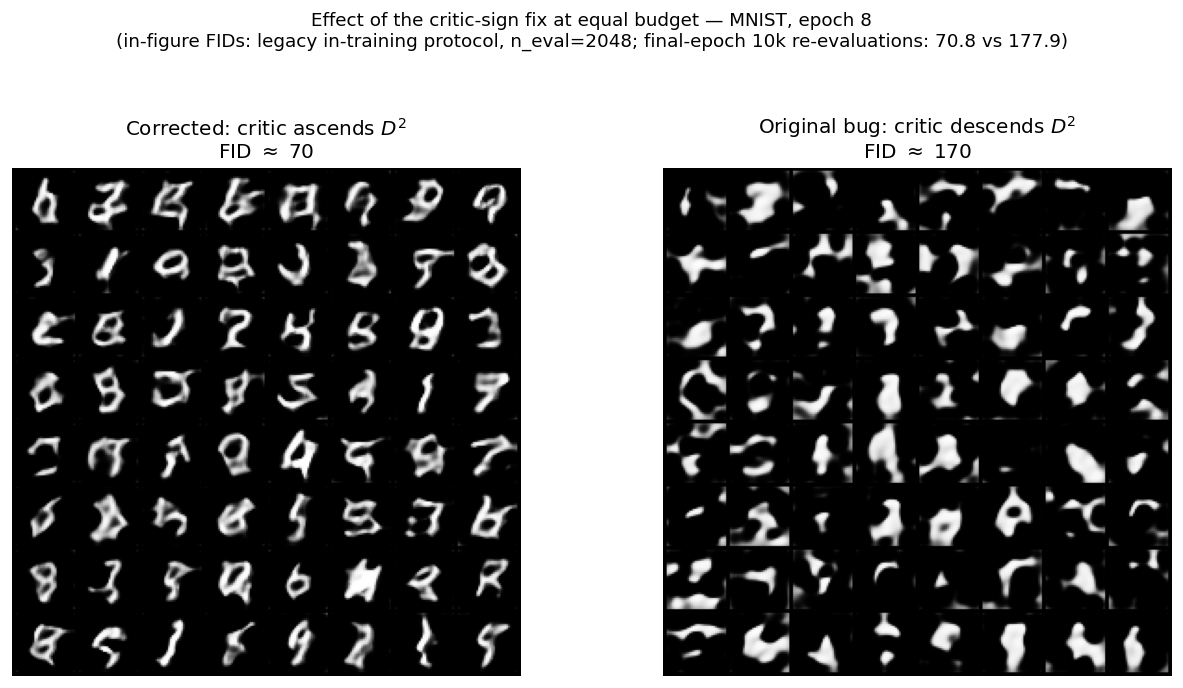
\includegraphics[width=0.86\textwidth]{figs/onoff_compare.png}
\caption{Effect of the critic-sign fix at equal budget (MNIST, epoch 8). \emph{Left}: the
corrected model (\texttt{critic\_sign=True}) produces clearly recognizable digits.
\emph{Right}: the original buggy direction (\texttt{critic\_sign=False}) produces only
blobs. The in-figure FID values are the legacy in-training evaluations
($n_{\mathrm{eval}}=2048$, epoch 8: $\approx 70$ vs.\ $\approx 170$); the final-epoch 10k
re-evaluations are 70.8 vs.\ 177.9.}
\label{fig:compare}
\end{figure*}

\section{Experiments and Results}

\subsection{Evaluation protocol}
\label{sec:protocol}
All models in this report are measured with \emph{one} evaluation harness: FID and KID on
10{,}000 generated versus 10{,}000 held-out test images (Inception-v3 features), plus a
domain-aware \emph{FID-LeNet} computed in the feature space of a LeNet classifier trained
on MNIST. The train-vs-test floor of this harness is FID 1.45 / FID-LeNet 1.76. Our
earlier ablation numbers were computed on $n=2048$ evaluation samples; since FID is
strongly biased at small $n$~\cite{chong2020}, we label those numbers \emph{legacy
protocol} and re-evaluate the final checkpoints at 10k. The Inception Score is kept only
as a sanity metric: it is essentially identical for the corrected and buggy models (2.33
vs.\ 2.34), i.e.\ uninformative on MNIST.

\subsection{Critic-sign ablation}
We train on the full MNIST training set for 18 epochs per run on an Apple-Silicon GPU (MPS),
with $\varepsilon=1$ and 50 Sinkhorn iterations. To isolate the central correction we run an
ablation on the critic direction (\texttt{critic\_sign} on vs.\ off) at equal budget;
quantitative results are reported in Table~\ref{tab:ablation}, the per-epoch FID in
Fig.~\ref{fig:fid}, and a qualitative comparison in Fig.~\ref{fig:compare}.

\begin{table}[h]
\centering
\footnotesize
\setlength{\tabcolsep}{3.5pt}
\resizebox{\columnwidth}{!}{%
\begin{tabular}{lccccc}
\toprule
& \multicolumn{1}{c}{legacy ($n{=}2048$)} & \multicolumn{4}{c}{re-evaluation @10k} \\
\cmidrule(lr){2-2}\cmidrule(lr){3-6}
\texttt{critic\_sign} & FID final / best & FID & KID$\times 10^3$ & FID-LeNet & IS \\
\midrule
\textbf{True} (corrected) & \textbf{77.2} / \textbf{69.9} & \textbf{70.8} & \textbf{65.7} & \textbf{77.0} & 2.33 \\
False (original bug)      & 185.3 / $\sim$170 & 177.9 & 191.0 & 208.8 & 2.34 \\
\bottomrule
\end{tabular}}
\caption{Critic-sign ablation on MNIST (18 epochs). The left column is the legacy protocol
($n_{\mathrm{eval}}=2048$, per-epoch); the right block re-evaluates the same final
checkpoints at 10k samples. Correcting the critic direction divides the FID by
$\approx 2.5$, consistently across all three feature spaces, while the IS does not move.}
\label{tab:ablation}
\end{table}

\begin{figure}[h]
\centering
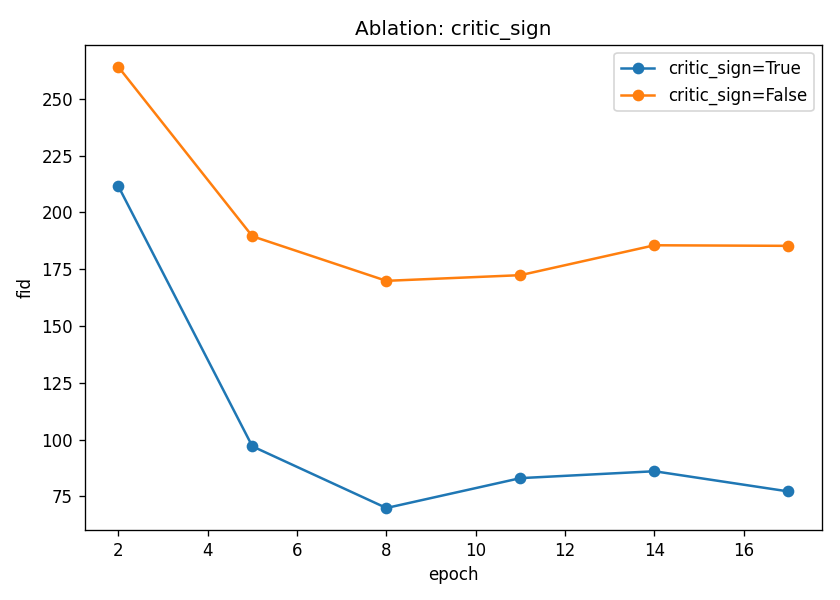
\includegraphics[width=0.95\linewidth]{figs/fid_ablation.png}
\caption{FID vs.\ epoch (legacy protocol, $n_{\mathrm{eval}}=2048$). The corrected run
(blue) stays well below the buggy run (orange) throughout, reaching its minimum
($\approx 70$) around epoch~8.}
\label{fig:fid}
\end{figure}

The corrected model produces clearly recognizable digits, a marked improvement over the
original report (whose samples were ``recognizable with more or less difficulty''). We also
observe that the best FID is reached mid-training (epoch~$\approx 8$): afterwards the energy
distance $D^2$ collapses toward~$0$ (a mild critic collapse) and the FID rises slightly, so
early stopping on the FID is advisable. The next subsection shows that this collapse is a
property of the \emph{objective}, not of the architecture.

\begin{figure*}[t]
\centering
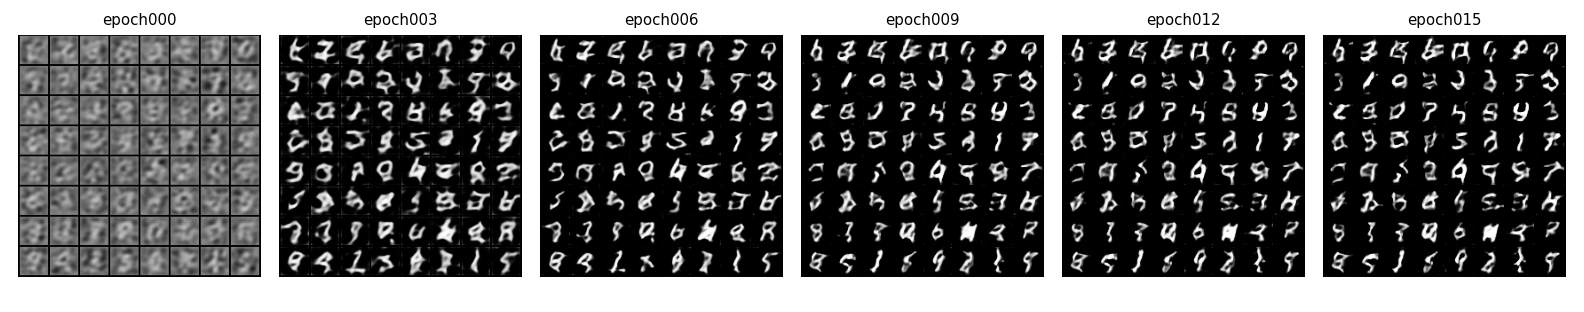
\includegraphics[width=0.95\textwidth]{figs/evolution_on.png}
\caption{Fixed-noise evolution of the corrected generator: the same latent codes are decoded
across epochs, showing the progression from noise to digits.}
\label{fig:evo}
\end{figure*}

\subsection{Modernized objective and 2024 successor}
\label{sec:modern}
As noted in Sec.~II, the mini-batch energy distance is exactly twice a Sinkhorn divergence
whose self-terms $\mathcal{W}(\mathbf{X},\mathbf{X}')$ use \emph{independent}
mini-batches. We therefore swap in the \emph{debiased} estimator of Feydy et
al.~\cite{feydy2019}---same-batch self-terms $\mathcal{W}(\mathbf{X},\mathbf{X})$---keeping
everything else identical: same architecture, same seed, same 8-epoch budget. The result
(Table~\ref{tab:loss}, Fig.~\ref{fig:loss}) is twofold: the FID drops from 81.2 to 24.4
(KID$\times 10^3$: 75.3 $\rightarrow$ 13.8), and the critic collapse documented above
\emph{disappears}---the training objective $D^2$ stays at $\approx 0.077$ instead of
collapsing to $\approx 10^{-4}$. The Sinkhorn-divergence run was still improving when the
budget ended.

\begin{table}[h]
\centering
\footnotesize
\setlength{\tabcolsep}{3.5pt}
\resizebox{\columnwidth}{!}{%
\begin{tabular}{lcccc}
\toprule
objective (8 epochs, same seed) & FID & KID$\times 10^3$ & FID-LeNet & final $D^2$ \\
\midrule
energy distance (2018) & 81.2 & 75.3 & 69.1 & $1.2\times 10^{-4}$ \\
Sinkhorn divergence (2019) & \textbf{24.4} & \textbf{13.8} & \textbf{60.1} & $0.077$ \\
\bottomrule
\end{tabular}}
\caption{Equal-budget loss comparison @10k samples. Debiasing the self-terms improves
every metric and removes the critic collapse (last column: the objective no longer
vanishes).}
\label{tab:loss}
\end{table}

\begin{figure*}[t]
\centering
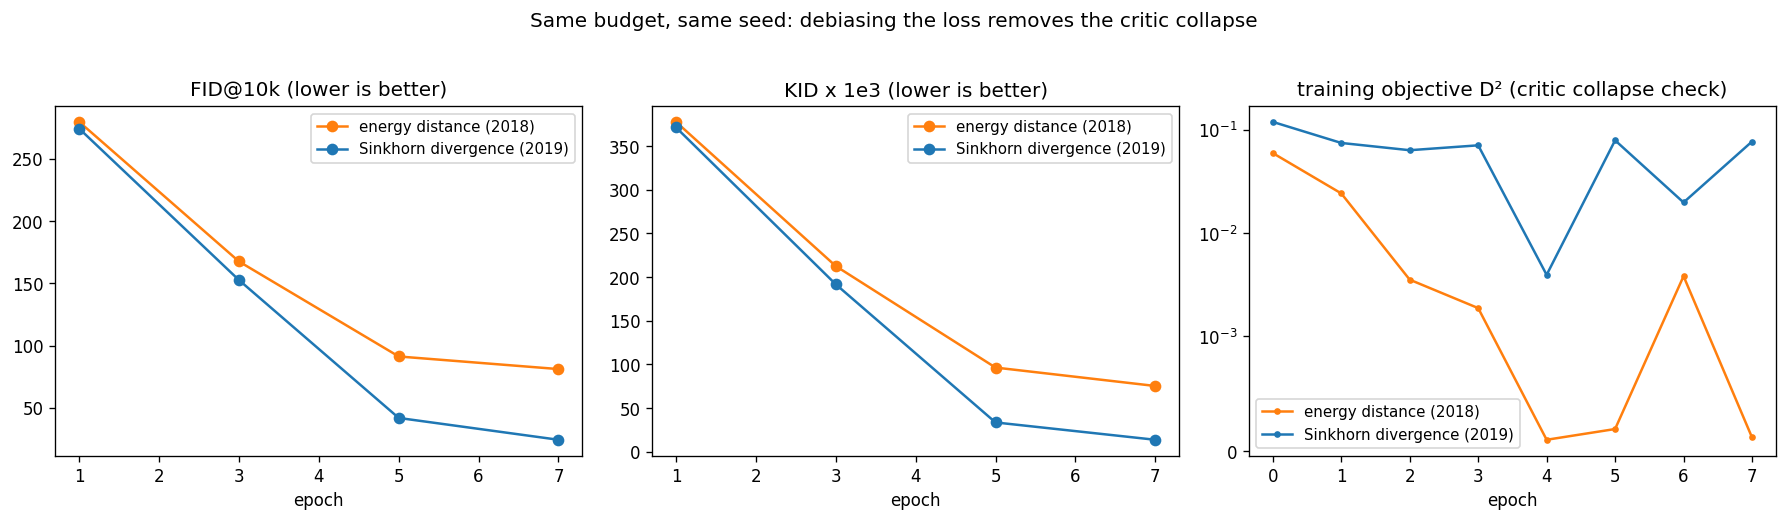
\includegraphics[width=0.95\textwidth]{figs/loss_comparison.png}
\caption{Same budget, same seed: debiasing the loss removes the critic collapse.
\emph{Left, middle}: FID@10k and KID$\times 10^3$ per epoch. \emph{Right}: the training
objective $D^2$ (log scale) collapses to $\approx 10^{-4}$ under the 2018 energy distance
but stays near $10^{-1}$ under the debiased Sinkhorn divergence.}
\label{fig:loss}
\end{figure*}

Finally, we implement the 2024 successor of this line of work: optimal-transport
conditional flow matching (OT-CFM)~\cite{tong2024,lipman2023}, reusing the \emph{same}
log-domain Sinkhorn solver to couple noise and data mini-batches---no critic, no minimax,
a single regression loss. Table~\ref{tab:headline} places all models under the single
harness of Sec.~\ref{sec:protocol}, together with a DCGAN calibration baseline and an
I-CFM control (independent pairs, \texttt{cfm\_coupling=none}) at identical capacity and
budget. The control matches OT-CFM at both 100 and 10 Euler sampling steps (FID 10.9 /
13.3 vs.\ 11.1 / 13.5 on best checkpoints): at this scale---mini-batch plans over 256
MNIST images---the OT coupling is an honest null result, consistent with its gains
concentrating in trajectory straightness, very-low-NFE regimes and harder datasets.
Ten-step sampling costs only $\approx$\,$+2.7$ FID over the 50-step sweet spot (10.8),
though in LeNet feature space ten-step sampling degrades $\approx 2.5\times$ (34.6 vs.\
13.6); note also that the GAN generator samples in a single forward pass while the flow
pays \texttt{ode\_steps} forward passes per sample. Repeated evaluations of one
checkpoint differ by $\approx$\,$\pm 0.3$ FID.

\begin{table*}[t]
\centering
\small
\begin{tabular}{lccccc}
\toprule
model & budget (MPS) & FID & KID$\times 10^3$ & FID-LeNet & IS \\
\midrule
OT-GAN, buggy sign (18 ep) & $\sim$6 h & 177.9 & 191.0 & 208.8 & 2.34 \\
OT-GAN, corrected (18 ep)  & $\sim$6 h & 70.8 & 65.7 & 77.0 & 2.33 \\
OT-GAN, energy dist.\ (8 ep) & $\sim$3.5 h & 81.2 & 75.3 & 69.1 & 2.33 \\
OT-GAN, Sinkhorn div.\ (8 ep) & $\sim$3.5 h & 24.4 & 13.8 & 60.1 & 1.98 \\
DCGAN baseline (10 ep) & $\sim$15 min & 72.3 & 74.6 & 36.8 & 2.19 \\
I-CFM, no coupling (30 ep) & $\sim$1.2 h & \textbf{10.9} & \textbf{8.9} & 12.8 & 1.91 \\
OT-CFM, Sinkhorn coupling (30 ep) & $\sim$1.2 h & 11.4 & 9.6 & \textbf{12.6} & 1.90 \\
\midrule
\emph{train-vs-test floor} & --- & 1.45 & --- & 1.76 & --- \\
\bottomrule
\end{tabular}
\caption{Headline results, all @10k samples under one harness. Flow matching, built on
the same Sinkhorn solver as the GANs, dominates both GAN families in a fraction of the
budget; the I-CFM control shows the mini-batch coupling itself is a wash at this scale.}
\label{tab:headline}
\end{table*}

For calibration: Lucic et al.~\cite{lucic2018} report MNIST FID $\approx 6.7$ (WGAN) and
$\approx 20.3$ (WGAN-GP) at much larger budgets with extensive hyperparameter search.
None of our numbers are state-of-the-art claims; they are \emph{controlled comparisons}
under one harness at laptop budgets. Note also that FID and FID-LeNet \emph{disagree} on
the DCGAN row (72.3 vs.\ 36.8, against 70.8 vs.\ 77.0 for the corrected OT-GAN): the
domain-aware metric ranks DCGAN clearly better while Inception-FID calls it a tie---itself
evidence that ImageNet-Inception features are unreliable on MNIST.

\section{From Images to Markets}
\label{sec:finance}
Nothing in the OT machinery above is image-specific. We close the experimental part
with two finance applications that reuse the \emph{same} log-domain Sinkhorn solver
and the \emph{same} training machinery on market data; both ship as executed
notebooks under \texttt{examples/}, which constitute the full artifacts.

\paragraph{Scenario reduction (no training).} Compressing a Monte Carlo book---turning
10{,}000 simulated paths into $K$ weighted scenarios whose mean, quantiles and CVaR
match the full set---is itself an optimal-transport problem. We solve it with an
entropic Lloyd iteration (``Sinkhorn $k$-means''): the plan is computed by the very
solver that trains the GAN, centroids are updated by barycentric projection, and as
$\varepsilon \to 0$ the plan hardens to nearest-scenario assignment, recovering
classical scenario reduction. The squared-Euclidean cost matrix is normalized
($C \leftarrow C/\mathrm{mean}(C)$) so that $\varepsilon$ is \emph{dimensionless} and
comparable with the $\varepsilon=1$ used on cosine costs; reduction runs near the
hard limit ($\varepsilon=0.01$). On a 20{,}000-path book (10k GBM + 10k Heston paths,
64 daily steps), fitted on one half with all risk statistics evaluated on the held-out half, $K=100$
scenarios reach a (fit-half) transport distortion of $0.008792$, against $0.008866$ for $k$-means and
$0.012031$ for random subsampling ($\approx 37\%$ worse). Both centroid methods place
the terminal mean correctly ($+0.0095$ vs.\ $+0.0058$ held out) but honestly
\emph{understate the tails}: $\mathrm{CVaR}_{95}$ $0.080$ vs.\ $0.221$ held out, with
$k$-means suffering identically (CVaR fidelity is a tie---OT slightly closer at
95\%, $k$-means at 99\%). This contraction is Jensen's inequality applied to
within-cluster averaging, not a solver artifact: the random subsample keeps actual
paths, hence unbiased tails ($\mathrm{CVaR}_{95}$ $0.163$), at the price of
representing individual paths $\approx 37\%$ worse---the classical
accuracy-versus-tail-fidelity trade-off of scenario reduction.

\paragraph{Heavy-tailed returns generation.} A 1D OT-GAN mirrors the image pair
component by component---a GLU generator with a \emph{linear} output head
(log-returns are unbounded, unlike $\tanh$-bounded pixels) and a dilated-convolution
CReLU critic with an $\ell_2$-normalized embedding whose 45-lag receptive field can
see volatility clustering---trained with the \emph{same} \texttt{compute\_loss} and
critic-sign machinery on a seeded GJR-GARCH(1,1) target~\cite{glosten1993}, whose
asymmetry $\gamma>0$ produces a genuine leverage effect that symmetric GARCH lacks.
At a 5.5-minute CPU budget (500 of the configured 3{,}000 steps), every headline
stylized fact comes out with the correct \emph{sign} and an overshot
\emph{magnitude} (Table~\ref{tab:finance}); the near-zero long-lag rows (ACF of
$|r|$ and $r^2$ at lags 10--20) fluctuate around zero. A critic-free \emph{debiased}
Sinkhorn divergence on raw paths reads $0.0499$ against a same-process finite-sample
floor of $\approx 0.0096$, i.e.\ the run is visibly mid-flight. Most tellingly, the
critic-sign ablation of Table~\ref{tab:ablation} replays here in minutes: under
identical seed and budget, the buggy direction collapses the training objective to
$+0.0004$---it looks ``solved''---while its samples carry a lag-1 return
autocorrelation of $+0.94$ (smooth curves, not returns) versus $-0.002$ for the
corrected sign. Calibrating the magnitudes, not just the signs, of temporal
dependence is precisely what causal-transport and finance-specific architectures
target; this section gestures toward that literature (COT-GAN~\cite{xu2020}, Quant
GANs~\cite{wiese2020}) with the engine already in place.

\begin{table}[h]
\centering
\footnotesize
\begin{tabular}{lrr}
\toprule
statistic & target & generated \\
\midrule
excess kurtosis & $+0.9992$ & $+7.0719$ \\
ACF($r$) lag-1 & $-0.0123$ & $-0.0022$ \\
ACF($|r|$) lag-1 & $+0.0310$ & $+0.2679$ \\
ACF($r^2$) lag-1 & $+0.0308$ & $+0.1495$ \\
leverage corr lag-1 & $-0.0243$ & $-0.2926$ \\
\bottomrule
\end{tabular}
\caption{Stylized facts of the GJR-GARCH(1,1) target vs.\ the 1D OT-GAN at the
5.5-minute CPU budget: right signs (including the leverage asymmetry), overshot
magnitudes---the typical mid-training profile.}
\label{tab:finance}
\end{table}

\section{Limitations}
All results are single-seed at laptop budgets (minutes to hours: Apple-Silicon MPS for
the image runs, CPU for the finance runs), so the gaps we report are large but not
variance-qualified. ImageNet-Inception features are a
questionable basis for MNIST evaluation: the IS is identical for corrected and buggy
models (2.33 vs.\ 2.34) and FID/FID-LeNet disagree on the DCGAN ranking, which is why we
report three metrics rather than one. The legacy 18-epoch runs kept only final-epoch
checkpoints, so their 10k re-evaluations are final-epoch, not best-epoch, numbers. Our
per-pair transport cost is the biased primal entropic cost $\mathrm{Tr}[MC^\top]$ (as in
the original OT-GAN), not the dual-potential form of Feydy et al., so the per-pair terms
are not exactly debiased even when assembled as a Sinkhorn divergence. Finally, the
Sinkhorn-divergence run was still improving when its 8-epoch budget ended, so its 24.4 FID
understates what the objective can reach.

\section{Code and Reproducibility}
The code, configurations, tests and this report are available at
\url{https://github.com/dan-allouche-qf/optimal-transport-gan} (MIT license). Release
\texttt{v1.0.0} ships two weight files with published SHA256 checksums: the EMA generator
of the best Sinkhorn-divergence epoch (FID 24.4@10k) and the full OT-CFM checkpoint (FID
11.4@10k); both load through \texttt{otgan sample --ckpt}. Each claim maps to one command:
\texttt{otgan ablate -c configs/mnist.yaml --axis critic\_sign --override n\_epochs=18}
(Table~\ref{tab:ablation}),
\texttt{otgan train -c configs/mnist.yaml --override loss=sinkhorn\_divergence}
(Table~\ref{tab:loss}), and \texttt{otgan train -c configs/cfm\_mnist.yaml} (the OT-CFM
row of Table~\ref{tab:headline}). The finance track of Sec.~\ref{sec:finance} maps to
the two executed notebooks under \texttt{examples/} (its numbers are read off their
cell outputs) and to \texttt{configs/finance\_returns.yaml}. The package is covered by
212 tests (203 fast, 9 slow;
$\approx 92\%$ line coverage) run in four CI jobs.

\section{Conclusion}
A faithful but corrected re-implementation of OT-GAN turns a buggy, CUDA-only notebook into a
tested, device-portable package whose corrected critic objective is the decisive factor for
sample quality: fixing the critic direction alone divides the FID by $\approx 2.5$ on MNIST.
Reading the 2018 loss through the Sinkhorn-divergence lens then pays twice---debiasing the
self-terms improves the FID from 81 to 24 at equal budget \emph{and} removes the critic
collapse---and the same Sinkhorn solver, reused for mini-batch coupling, powers an OT-CFM
successor that reaches FID 11.4 in about an hour. Pointed at market data, the identical
engine compresses a 20{,}000-path Monte Carlo book into 100 weighted scenarios with
held-out risk fidelity and replays the critic-sign ablation on GJR-GARCH returns in
minutes. The full code, configurations, tests and
ablation harness are released alongside this report.

\begin{thebibliography}{99}
\bibitem{salimans2018} T.~Salimans, H.~Zhang, A.~Radford, and D.~Metaxas,
``Improving GANs using Optimal Transport,'' in \emph{ICLR}, 2018.
\bibitem{cuturi2013} M.~Cuturi,
``Sinkhorn Distances: Lightspeed Computation of Optimal Transport,'' in \emph{NeurIPS}, 2013.
\bibitem{genevay2018} A.~Genevay, G.~Peyr\'e, and M.~Cuturi,
``Learning Generative Models with Sinkhorn Divergences,'' in \emph{AISTATS}, 2018.
\bibitem{feydy2019} J.~Feydy, T.~S\'ejourn\'e, F.-X.~Vialard, S.~Amari, A.~Trouv\'e, and
G.~Peyr\'e, ``Interpolating between Optimal Transport and MMD using Sinkhorn Divergences,''
in \emph{AISTATS}, 2019.
\bibitem{lipman2023} Y.~Lipman, R.~T.~Q.~Chen, H.~Ben-Hamu, M.~Nickel, and M.~Le,
``Flow Matching for Generative Modeling,'' in \emph{ICLR}, 2023.
\bibitem{tong2024} A.~Tong, K.~Fatras, N.~Malkin, G.~Huguet, Y.~Zhang, J.~Rector-Brooks,
G.~Wolf, and Y.~Bengio, ``Improving and Generalizing Flow-Based Generative Models with
Minibatch Optimal Transport,'' \emph{TMLR}, 2024.
\bibitem{huang2024} Y.~Huang, A.~Gokaslan, V.~Kuleshov, and J.~Tompkin,
``The GAN is dead; long live the GAN! A Modern GAN Baseline,'' in \emph{NeurIPS}, 2024.
\bibitem{binkowski2018} M.~Bi\'nkowski, D.~J.~Sutherland, M.~Arbel, and A.~Gretton,
``Demystifying MMD GANs,'' in \emph{ICLR}, 2018.
\bibitem{parmar2022} G.~Parmar, R.~Zhang, and J.-Y.~Zhu,
``On Aliased Resizing and Surprising Subtleties in GAN Evaluation,'' in \emph{CVPR}, 2022.
\bibitem{chong2020} M.~J.~Chong and D.~Forsyth,
``Effectively Unbiased FID and Inception Score and Where to Find Them,'' in \emph{CVPR}, 2020.
\bibitem{lucic2018} M.~Lucic, K.~Kurach, M.~Michalski, S.~Gelly, and O.~Bousquet,
``Are GANs Created Equal? A Large-Scale Study,'' in \emph{NeurIPS}, 2018.
\bibitem{glosten1993} L.~R.~Glosten, R.~Jagannathan, and D.~E.~Runkle,
``On the Relation between the Expected Value and the Volatility of the Nominal Excess
Return on Stocks,'' \emph{The Journal of Finance}, vol.~48, no.~5, 1993.
\bibitem{xu2020} T.~Xu, L.~K.~Wenliang, M.~Munn, and B.~Acciaio,
``COT-GAN: Generating Sequential Data via Causal Optimal Transport,'' in
\emph{NeurIPS}, 2020.
\bibitem{wiese2020} M.~Wiese, R.~Knobloch, R.~Korn, and P.~Kretschmer,
``Quant GANs: Deep Generation of Financial Time Series,'' \emph{Quantitative Finance},
vol.~20, no.~9, 2020.
\end{thebibliography}

\end{document}
